%%%%%%%%%%%%%%%%%%%%%%%%%%%%%%%%%%%%%%%%%%%%%%%%%%%
%
%  New template code for TAMU Theses and Dissertations starting Fall 2012.  
%  For more info about this template or the 
%  TAMU LaTeX User's Group, see http://www.howdy.me/.
%
%  Author: Wendy Lynn Turner 
%	 Version 1.0 
%  Last updated 8/5/2012
%
%%%%%%%%%%%%%%%%%%%%%%%%%%%%%%%%%%%%%%%%%%%%%%%%%%%

%%%%%%%%%%%%%%%%%%%%%%%%%%%%%%%%%%%%%%%%%%%%%%%%%%%%%%%%%%%%%%%%%%%%%%
%%                           APPENDIX A 
%%%%%%%%%%%%%%%%%%%%%%%%%%%%%%%%%%%%%%%%%%%%%%%%%%%%%%%%%%%%%%%%%%%%%

\phantomsection

\chapter{\uppercase{MS Observations}}

\begin{figure}
\begin{center}
	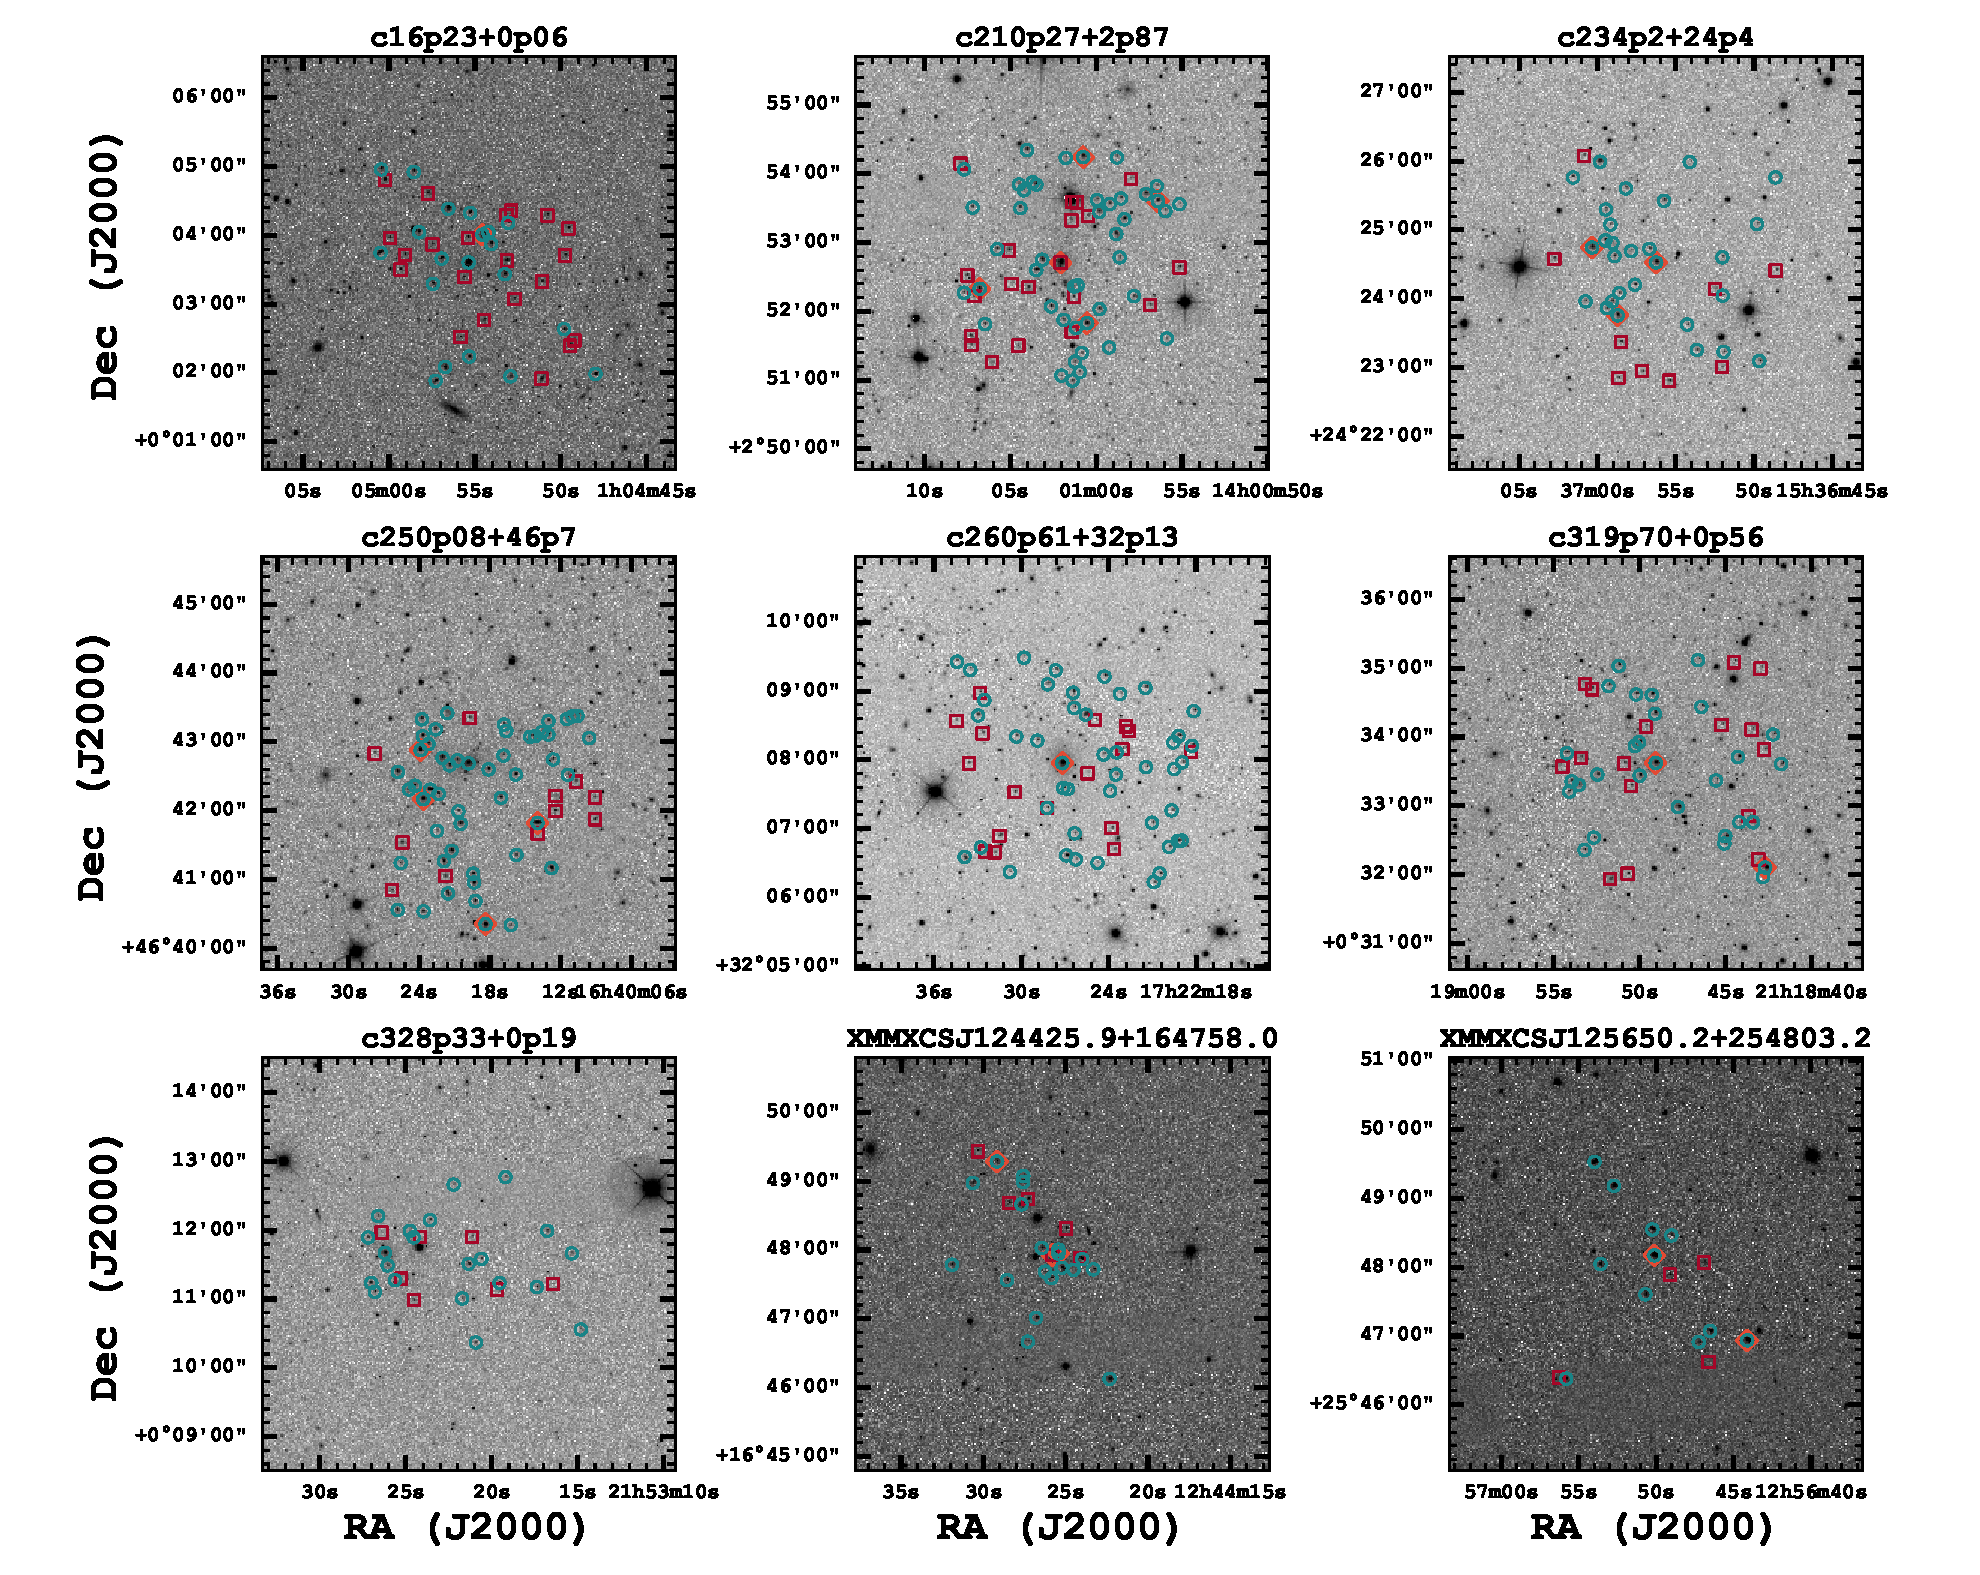
\includegraphics[width=\textwidth]{./figures2/multimontage.pdf}
\end{center}
	\caption[Montage of remaining nine clusters]{SDSS \sdssr\ image of cluster c203p83+41p0. The symbols show the position of observed galaxies. Blue circles indicate galaxies with $Q=0$ or $Q=1$ spectroscopic redshifts, red squares indicate galaxies where a redshift could not be reliably determined, and the orange diamond corresponds to galaxies with pre-existing redshifts from the SDSS. \textit{Right:} Example spectrum of an emission-line cluster galaxy (black line) and template fit (red line) from VIRUS-P on the McDonald 2.7m telescope. The spectrum shows the wavelength range and data quality expected from HETDEX-like spectroscopy, which are sufficient to measure galaxy redshifts.} 
	\label{fig:montage}
\end{figure}


\begin{landscape}
	\begin{table}
		\centering 
		\caption[Spectroscopic redshifts for galaxies in c16p23+0p06.]{Spectroscopic redshifts for galaxies in c16p23+0p06: Columns as in Table~\ref{2tbl:c203p83+41p0}.}
		\begin{tabular}{ccccccccccc}
			\hline
			tile & dither & fiber & ra & dec & r (mag) & redshift & Q & Member & R (Mpc) & LOSV (\kms) \\
			(1) & (2) & (3) & (4) & (5) & (6) & (7) & (8) & (9) & (10) & (11) \\
			\hline \hline
			NE & 1 & 223 & 01:04:56.937 & +00:03:39.60 & 19.38 & 0.2691$\pm{0.0002}$ & 0 & $\checkmark$ & 0.10 & -748$\pm{89}$ \\
			NE & 2 & 42 & 01:05:00.449 & +00:04:57.41 & 19.80 & 0.2766$\pm{0.0001}$ & 1 & $\checkmark$ & 0.47 & 1005$\pm{52}$ \\
			NE & 2 & 168 & 01:04:58.247 & +00:04:02.62 & 19.75 & 0.3054$\pm{0.0003}$ & 1 & ... & 0.23 & 7783$\pm{122}$ \\
			NE & 2 & 216 & 01:05:00.487 & +00:03:44.70 & 18.85 & 0.0826$\pm{0.0004}$ & 1 & ... & 0.12 & -44576$\pm{193}$ \\
			NE & 2 & 220 & 01:04:55.367 & +00:03:36.34 & 17.27 & 0.2715$\pm{0.0001}$ & 0 & $\checkmark$ & 0.00 & -193$\pm{61}$ \\
			NE & 3 & 38 & 01:04:58.559 & +00:04:55.13 & 19.95 & 0.3510$\pm{0.0001}$ & 1 & ... & 0.46 & 18494$\pm{56}$ \\
			NE & 3 & 106 & 01:04:56.545 & +00:04:23.15 & 18.36 & 0.2788$\pm{0.0001}$ & 0 & $\checkmark$ & 0.21 & 1517$\pm{47}$ \\
			NE & 3 & 118 & 01:04:55.276 & +00:04:19.53 & 19.49 & 0.2747$\pm{0.0001}$ & 0 & $\checkmark$ & 0.18 & 566$\pm{71}$ \\
			NE & 3 & 160 & 01:04:54.563 & +00:04:00.66 & 18.19 & 0.2747$\pm{0.0001}$ & 0 & $\checkmark$ & 0.11 & 559$\pm{52}$ \\
			NW & 1 & 156 & 01:04:53.064 & +00:04:10.99 & 20.22 & 0.2234$\pm{0.0001}$ & 1 & ... & 0.18 & -11495$\pm{52}$ \\
			NW & 2 & 173 & 01:04:54.217 & +00:04:02.78 & 19.62 & 0.2629$\pm{0.0002}$ & 0 & $\checkmark$ & 0.13 & -2205$\pm{80}$ \\
			NW & 3 & 187 & 01:04:54.051 & +00:03:52.42 & 19.35 & 0.3290$\pm{0.0001}$ & 1 & ... & 0.12 & 13319$\pm{52}$ \\
			SE & 1 & 50 & 01:04:57.440 & +00:03:17.71 & 19.51 & 0.2718$\pm{0.0002}$ & 1 & $\checkmark$ & 0.15 & -123$\pm{75}$ \\
			SE & 2 & 191 & 01:04:55.332 & +00:02:14.18 & 19.79 & 0.2794$\pm{0.0001}$ & 0 & $\checkmark$ & 0.35 & 1658$\pm{66}$ \\
			SE & 3 & 208 & 01:04:56.734 & +00:02:05.07 & 18.75 & 0.2781$\pm{0.0001}$ & 0 & $\checkmark$ & 0.40 & 1358$\pm{42}$ \\
			SE & 3 & 238 & 01:04:57.284 & +00:01:53.04 & 19.58 & 0.2705$\pm{0.0001}$ & 0 & $\checkmark$ & 0.45 & -421$\pm{66}$ \\
			SW & 2 & 26 & 01:04:53.268 & +00:03:26.04 & 18.99 & 0.2666$\pm{0.0002}$ & 0 & $\checkmark$ & 0.14 & -1352$\pm{85}$ \\
			SW & 2 & 135 & 01:04:49.814 & +00:02:38.18 & 20.10 & 0.2697$\pm{0.0002}$ & 1 & $\checkmark$ & 0.42 & -619$\pm{85}$ \\
			SW & 2 & 218 & 01:04:47.988 & +00:01:59.05 & 19.55 & 0.2627$\pm{0.0001}$ & 1 & $\checkmark$ & 0.60 & -2259$\pm{42}$ \\
			SW & 3 & 228 & 01:04:52.934 & +00:01:56.95 & 20.37 & 0.2763$\pm{0.0001}$ & 1 & $\checkmark$ & 0.45 & 928$\pm{47}$ \\
			\hline
		\end{tabular}
		\label{2tbl:c16p23+0p06}
	\end{table}
\end{landscape}


\begin{landscape}
	\singlespace
	\begin{longtable}{ccccccccccc}
	\caption[Spectroscopic redshifts for galaxies in c234p2+24p4.]{Spectroscopic redshifts for galaxies in c234p2+24p4: Columns as in Table~\ref{2tbl:c203p83+41p0}.}\\
	\hline
	tile & dither & fiber & ra & dec & r (mag) & redshift & Q & Member & R (Mpc) & LOSV (\kms) \\
	(1) & (2) & (3) & (4) & (5) & (6) & (7) & (8) & (9) & (10) & (11) \\
	\hline \hline
	\endfirsthead
	\multicolumn{4}{l}%
	{\tablename\ \thetable\ Continued} \\
	\hline
	tile & dither & fiber & ra & dec & r (mag) & redshift & Q & Member & R (Mpc) & LOSV (\kms) \\
	(1) & (2) & (3) & (4) & (5) & (6) & (7) & (8) & (9) & (10) & (11) \\
	\hline \hline
	\endhead
	NE & 1 & 78 & 15:36:58.192 & +24:25:36.14 & 19.81 & 0.3228$\pm{0.0001}$ & 0 & ... & 0.33 & 23652$\pm{44}$ \\
	NE & 1 & 124 & 15:36:59.468 & +24:25:17.76 & 19.83 & 0.2324$\pm{0.0004}$ & 1 & $\checkmark$ & 0.24 & 1609$\pm{195}$ \\
	NE & 1 & 208 & 15:36:57.848 & +24:24:41.47 & 20.35 & 0.1881$\pm{0.0001}$ & 0 & ... & 0.08 & -9197$\pm{34}$ \\
	NE & 2 & 11 & 15:37:00.861 & +24:26:04.40 & 20.48 & 0.0947$\pm{0.0001}$ & 1 & ... & 0.20 & -31965$\pm{54}$ \\
	NE & 2 & 153 & 15:36:59.174 & +24:25:04.55 & 20.37 & 0.1036$\pm{0.0002}$ & 1 & ... & 0.10 & -29809$\pm{98}$ \\
	NE & 2 & 232 & 15:37:02.759 & +24:24:34.63 & 19.98 & 0.3017$\pm{0.0001}$ & 1 & ... & 0.40 & 18513$\pm{49}$ \\
	NE & 3 & 23 & 15:36:59.839 & +24:25:59.51 & 18.05 & 0.1275$\pm{0.0000}$ & 0 & ... & 0.23 & -23979$\pm{20}$ \\
	NE & 3 & 55 & 15:37:01.554 & +24:25:45.67 & 19.79 & 0.2115$\pm{0.0001}$ & 1 & ... & 0.36 & -3477$\pm{49}$ \\
	NE & 3 & 181 & 15:36:59.035 & +24:24:48.56 & 20.11 & 0.1874$\pm{0.0001}$ & 1 & ... & 0.13 & -9363$\pm{39}$ \\
	NE & 3 & 182 & 15:36:59.498 & +24:24:50.78 & 19.62 & 0.1231$\pm{0.0003}$ & 1 & ... & 0.11 & -25050$\pm{151}$ \\
	NE & 3 & 191 & 15:36:56.681 & +24:24:43.40 & 19.54 & 0.1808$\pm{0.0000}$ & 0 & ... & 0.04 & -10980$\pm{24}$ \\
	NE & 3 & 198 & 15:37:00.334 & +24:24:44.60 & 17.27 & 0.2274$\pm{0.0002}$ & 0 & $\checkmark$ & 0.21 & 387$\pm{112}$ \\
	NE & 3 & 210 & 15:36:58.911 & +24:24:37.07 & 19.67 & 0.4813$\pm{0.0000}$ & 1 & ... & 0.22 & 62324$\pm{24}$ \\
	NE & 3 & 219 & 15:36:56.253 & +24:24:31.59 & 17.36 & 0.2262$\pm{0.0001}$ & 0 & $\checkmark$ & 0.00 & 94$\pm{63}$ \\
	NW & 1 & 116 & 15:36:55.756 & +24:25:25.38 & 18.90 & 0.2706$\pm{0.0001}$ & 1 & ... & 0.23 & 10924$\pm{49}$ \\
	NW & 1 & 148 & 15:36:49.817 & +24:25:04.96 & 20.02 & 0.2224$\pm{0.0001}$ & 0 & $\checkmark$ & 0.34 & -813$\pm{63}$ \\
	NW & 2 & 26 & 15:36:54.106 & +24:25:59.10 & 20.79 & 0.2298$\pm{0.0000}$ & 0 & $\checkmark$ & 0.34 & 972$\pm{24}$ \\
	NW & 3 & 44 & 15:36:48.628 & +24:25:45.78 & 21.29 & 0.3341$\pm{0.0001}$ & 1 & ... & 0.62 & 26416$\pm{59}$ \\
	NW & 3 & 210 & 15:36:52.024 & +24:24:36.09 & 19.78 & 0.2281$\pm{0.0001}$ & 0 & $\checkmark$ & 0.21 & 570$\pm{63}$ \\
	SE & 1 & 48 & 15:36:57.612 & +24:24:12.18 & 19.43 & 0.2215$\pm{0.0002}$ & 0 & $\checkmark$ & 0.10 & -1038$\pm{78}$ \\
	SE & 1 & 64 & 15:36:58.605 & +24:24:04.80 & 20.06 & 0.2124$\pm{0.0001}$ & 1 & ... & 0.15 & -3277$\pm{59}$ \\
	SE & 2 & 80 & 15:36:59.058 & +24:23:57.63 & 19.24 & 0.2280$\pm{0.0002}$ & 0 & $\checkmark$ & 0.19 & 528$\pm{93}$ \\
	SE & 2 & 95 & 15:36:59.393 & +24:23:51.85 & 19.35 & 0.1244$\pm{0.0002}$ & 1 & ... & 0.13 & -24730$\pm{98}$ \\
	SE & 3 & 108 & 15:36:58.708 & +24:23:45.47 & 17.70 & 0.2235$\pm{0.0002}$ & 0 & $\checkmark$ & 0.21 & -565$\pm{83}$ \\
	SW & 1 & 66 & 15:36:52.487 & +24:24:08.35 & 20.29 & 0.1248$\pm{0.0001}$ & 1 & ... & 0.13 & -24633$\pm{63}$ \\
	SW & 1 & 142 & 15:36:54.270 & +24:23:37.37 & 20.15 & 0.2546$\pm{0.0001}$ & 0 & ... & 0.24 & 7019$\pm{54}$ \\
	SW & 2 & 185 & 15:36:53.657 & +24:23:15.33 & 19.58 & 0.2239$\pm{0.0002}$ & 0 & $\checkmark$ & 0.30 & -450$\pm{98}$ \\
	SW & 3 & 65 & 15:36:51.996 & +24:24:02.62 & 20.31 & 0.2201$\pm{0.0001}$ & 1 & $\checkmark$ & 0.23 & -1382$\pm{34}$ \\
	\hline
	\label{2tbl:c234p2+24p4}
	\end{longtable}
\end{landscape}


\begin{landscape}
	\singlespace
	\begin{longtable}{ccccccccccc}
	\caption[Spectroscopic redshifts for galaxies in c250p08+46p7]{Spectroscopic redshifts for galaxies in c250p08+46p7: Columns as in Table~\ref{2tbl:c203p83+41p0}.}\\
	\hline
	tile & dither & fiber & ra & dec & r (mag) & redshift & Q & Member & R (Mpc) & LOSV (\kms) \\
	(1) & (2) & (3) & (4) & (5) & (6) & (7) & (8) & (9) & (10) & (11) \\
	\hline \hline
	\endfirsthead
	\multicolumn{4}{l}%
	{\tablename\ \thetable\ Continued} \\
	\hline
	tile & dither & fiber & ra & dec & r (mag) & redshift & Q & Member & R (Mpc) & LOSV (\kms) \\
	(1) & (2) & (3) & (4) & (5) & (6) & (7) & (8) & (9) & (10) & (11) \\
	\hline \hline
	\endhead
	NE & 1 & 34 & 16:40:21.617 & +46:43:25.07 & 20.12 & 0.1014$\pm{0.0003}$ & 0 & ... & 0.09 & -30528$\pm{141}$ \\
	NE & 1 & 110 & 16:40:23.879 & +46:42:52.76 & 17.81 & 0.2333$\pm{0.0000}$ & 0 & $\checkmark$ & 0.16 & 1617$\pm{24}$ \\
	NE & 1 & 133 & 16:40:19.812 & +46:42:41.30 & 16.61 & 0.2238$\pm{0.0001}$ & 0 & $\checkmark$ & 0.00 & -699$\pm{39}$ \\
	NE & 1 & 156 & 16:40:25.818 & +46:42:33.87 & 18.36 & 0.2099$\pm{0.0001}$ & 0 & ... & 0.21 & -4092$\pm{54}$ \\
	NE & 1 & 183 & 16:40:24.352 & +46:42:21.79 & 19.33 & 0.2248$\pm{0.0002}$ & 0 & $\checkmark$ & 0.18 & -462$\pm{93}$ \\
	NE & 1 & 211 & 16:40:23.651 & +46:42:10.01 & 17.62 & 0.2287$\pm{0.0001}$ & 0 & $\checkmark$ & 0.19 & 483$\pm{39}$ \\
	NE & 2 & 65 & 16:40:22.597 & +46:43:10.93 & 19.73 & 0.1813$\pm{0.0002}$ & 1 & ... & 0.13 & -11053$\pm{88}$ \\
	NE & 2 & 81 & 16:40:23.696 & +46:43:04.86 & 18.62 & 0.2324$\pm{0.0001}$ & 0 & $\checkmark$ & 0.17 & 1400$\pm{68}$ \\
	NE & 2 & 95 & 16:40:23.219 & +46:42:58.04 & 19.32 & 0.2264$\pm{0.0001}$ & 0 & $\checkmark$ & 0.14 & -75$\pm{39}$ \\
	NE & 2 & 122 & 16:40:22.018 & +46:42:46.03 & 18.84 & 0.2079$\pm{0.0001}$ & 0 & ... & 0.08 & -4574$\pm{73}$ \\
	NE & 2 & 136 & 16:40:21.428 & +46:42:39.59 & 19.11 & 0.2180$\pm{0.0002}$ & 0 & $\checkmark$ & 0.06 & -2120$\pm{93}$ \\
	NE & 2 & 195 & 16:40:22.346 & +46:42:14.63 & 19.21 & 0.2289$\pm{0.0002}$ & 0 & $\checkmark$ & 0.14 & 542$\pm{93}$ \\
	NE & 3 & 37 & 16:40:23.777 & +46:43:19.71 & 19.22 & 0.2229$\pm{0.0002}$ & 0 & $\checkmark$ & 0.20 & -933$\pm{102}$ \\
	NE & 3 & 120 & 16:40:20.755 & +46:42:43.96 & 17.82 & 0.2216$\pm{0.0002}$ & 0 & $\checkmark$ & 0.04 & -1240$\pm{83}$ \\
	NE & 3 & 181 & 16:40:23.067 & +46:42:18.32 & 18.39 & 0.2191$\pm{0.0001}$ & 0 & $\checkmark$ & 0.14 & -1852$\pm{39}$ \\
	NE & 3 & 184 & 16:40:24.861 & +46:42:18.39 & 19.09 & 0.2110$\pm{0.0002}$ & 0 & ... & 0.20 & -3816$\pm{78}$ \\
	NW & 1 & 50 & 16:40:13.038 & +46:43:18.14 & 19.37 & 0.2289$\pm{0.0002}$ & 0 & $\checkmark$ & 0.29 & 539$\pm{78}$ \\
	NW & 1 & 79 & 16:40:13.042 & +46:43:06.31 & 19.12 & 0.2297$\pm{0.0001}$ & 0 & $\checkmark$ & 0.27 & 730$\pm{34}$ \\
	NW & 1 & 81 & 16:40:14.572 & +46:43:04.50 & 20.49 & 0.2249$\pm{0.0002}$ & 1 & $\checkmark$ & 0.21 & -443$\pm{102}$ \\
	NW & 1 & 128 & 16:40:16.854 & +46:42:48.04 & 20.31 & 0.2281$\pm{0.0001}$ & 1 & $\checkmark$ & 0.11 & 342$\pm{68}$ \\
	NW & 1 & 215 & 16:40:17.060 & +46:42:11.27 & 19.21 & 0.2580$\pm{0.0002}$ & 1 & ... & 0.17 & 7632$\pm{122}$ \\
	NW & 2 & 33 & 16:40:10.991 & +46:43:22.18 & 19.33 & 0.2228$\pm{0.0001}$ & 1 & $\checkmark$ & 0.36 & -940$\pm{49}$ \\
	NW & 2 & 56 & 16:40:16.794 & +46:43:15.13 & 20.91 & 0.2350$\pm{0.0001}$ & 1 & $\checkmark$ & 0.17 & 2021$\pm{73}$ \\
	NW & 2 & 70 & 16:40:16.608 & +46:43:09.56 & 20.70 & 0.2167$\pm{0.0002}$ & 1 & $\checkmark$ & 0.15 & -2427$\pm{88}$ \\
	NW & 2 & 81 & 16:40:14.180 & +46:43:05.00 & 19.20 & 0.2252$\pm{0.0001}$ & 0 & $\checkmark$ & 0.23 & -375$\pm{68}$ \\
	NW & 2 & 156 & 16:40:15.807 & +46:42:31.47 & 18.88 & 0.2281$\pm{0.0002}$ & 0 & $\checkmark$ & 0.16 & 344$\pm{83}$ \\
	NW & 3 & 33 & 16:40:11.463 & +46:43:19.95 & 19.11 & 0.2249$\pm{0.0002}$ & 0 & $\checkmark$ & 0.34 & -426$\pm{97}$ \\
	NW & 3 & 65 & 16:40:13.553 & +46:43:08.81 & 20.49 & 0.1319$\pm{0.0001}$ & 1 & ... & 0.16 & -23097$\pm{29}$ \\
	NW & 3 & 74 & 16:40:09.583 & +46:43:03.29 & 20.34 & 0.1735$\pm{0.0001}$ & 1 & ... & 0.32 & -12967$\pm{58}$ \\
	NW & 3 & 122 & 16:40:12.635 & +46:42:44.68 & 19.66 & 0.2270$\pm{0.0001}$ & 0 & $\checkmark$ & 0.27 & 79$\pm{63}$ \\
	NW & 3 & 144 & 16:40:18.116 & +46:42:35.97 & 19.27 & 0.2080$\pm{0.0002}$ & 1 & ... & 0.06 & -4567$\pm{102}$ \\
	NW & 3 & 149 & 16:40:11.390 & +46:42:31.31 & 20.02 & 0.0844$\pm{0.0002}$ & 1 & ... & 0.14 & -34675$\pm{88}$ \\
	SE & 1 & 4 & 16:40:20.674 & +46:41:59.40 & 20.48 & 0.2341$\pm{0.0001}$ & 0 & $\checkmark$ & 0.16 & 1797$\pm{54}$ \\
	SE & 1 & 50 & 16:40:22.486 & +46:41:42.33 & 20.51 & 0.2376$\pm{0.0002}$ & 1 & ... & 0.25 & 2670$\pm{78}$ \\
	SE & 1 & 107 & 16:40:21.903 & +46:41:15.96 & 18.82 & 0.1866$\pm{0.0001}$ & 0 & ... & 0.28 & -9766$\pm{58}$ \\
	SE & 1 & 147 & 16:40:19.343 & +46:40:57.31 & 18.39 & 0.1864$\pm{0.0001}$ & 0 & ... & 0.33 & -9815$\pm{34}$ \\
	SE & 1 & 211 & 16:40:23.625 & +46:40:32.22 & 19.06 & 0.2325$\pm{0.0001}$ & 0 & $\checkmark$ & 0.50 & 1410$\pm{54}$ \\
	SE & 1 & 214 & 16:40:25.819 & +46:40:33.21 & 19.03 & 0.2272$\pm{0.0002}$ & 0 & $\checkmark$ & 0.52 & 113$\pm{93}$ \\
	SE & 2 & 113 & 16:40:25.565 & +46:41:14.28 & 20.51 & 0.2221$\pm{0.0002}$ & 0 & $\checkmark$ & 0.38 & -1116$\pm{83}$ \\
	SE & 2 & 165 & 16:40:21.553 & +46:40:47.83 & 18.59 & 0.2110$\pm{0.0001}$ & 1 & ... & 0.40 & -3819$\pm{68}$ \\
	SE & 3 & 18 & 16:40:20.484 & +46:41:48.57 & 18.80 & 0.2347$\pm{0.0001}$ & 0 & $\checkmark$ & 0.20 & 1960$\pm{58}$ \\
	SE & 3 & 77 & 16:40:21.250 & +46:41:25.01 & 18.21 & 0.1892$\pm{0.0001}$ & 0 & ... & 0.25 & -9128$\pm{29}$ \\
	SE & 3 & 118 & 16:40:19.417 & +46:41:05.03 & 19.40 & 0.2238$\pm{0.0002}$ & 0 & $\checkmark$ & 0.35 & -701$\pm{102}$ \\
	SE & 3 & 176 & 16:40:19.231 & +46:40:41.13 & 19.36 & 0.2167$\pm{0.0001}$ & 0 & ... & 0.42 & -2444$\pm{39}$ \\
	SW & 1 & 122 & 16:40:12.787 & +46:41:09.93 & 18.22 & 0.2340$\pm{0.0001}$ & 0 & $\checkmark$ & 0.44 & 1785$\pm{34}$ \\
	SW & 1 & 243 & 16:40:16.232 & +46:40:20.20 & 20.28 & 0.2278$\pm{0.0002}$ & 1 & $\checkmark$ & 0.53 & 274$\pm{88}$ \\
	SW & 1 & 246 & 16:40:18.377 & +46:40:20.93 & 17.51 & 0.1874$\pm{0.0002}$ & 0 & ... & 0.44 & -9576$\pm{107}$ \\
	SW & 2 & 98 & 16:40:15.754 & +46:41:21.37 & 20.03 & 0.2243$\pm{0.0001}$ & 0 & $\checkmark$ & 0.33 & -572$\pm{63}$ \\
	SW & 3 & 22 & 16:40:13.962 & +46:41:49.44 & 17.63 & 0.1107$\pm{0.0001}$ & 0 & ... & 0.16 & -28264$\pm{54}$ \\
	\hline
	\label{2tbl:c250p08+46p7}
	\end{longtable}
\end{landscape}


\begin{landscape}
	\singlespace
	\begin{longtable}{ccccccccccc}
	\caption[Spectroscopic redshifts for galaxies in c210p27+2p87]{Spectroscopic redshifts for galaxies in c210p27+2p87: Columns as in Table~\ref{2tbl:c203p83+41p0}.}\\
	\hline
	tile & dither & fiber & ra & dec & r (mag) & redshift & Q & Member & R (Mpc) & LOSV (\kms) \\
	(1) & (2) & (3) & (4) & (5) & (6) & (7) & (8) & (9) & (10) & (11) \\
	\hline \hline
	\endfirsthead
	\multicolumn{4}{l}%
	{\tablename\ \thetable\ Continued} \\
	\hline
	tile & dither & fiber & ra & dec & r (mag) & redshift & Q & Member & R (Mpc) & LOSV (\kms) \\
	(1) & (2) & (3) & (4) & (5) & (6) & (7) & (8) & (9) & (10) & (11) \\
	\hline \hline
	\endhead
	NE & 1 & 6 & 14:01:04.022 & +02:54:20.65 & 19.01 & 0.2478$\pm{0.0002}$ & 0 & $\checkmark$ & 0.40 & -1626$\pm{81}$ \\
	NE & 1 & 16 & 14:01:01.771 & +02:54:13.80 & 20.37 & 0.3158$\pm{0.0002}$ & 1 & ... & 0.42 & 14574$\pm{81}$ \\
	NE & 1 & 123 & 14:01:04.410 & +02:53:29.95 & 19.70 & 0.2325$\pm{0.0002}$ & 1 & ... & 0.22 & -5275$\pm{119}$ \\
	NE & 2 & 43 & 14:01:07.682 & +02:54:03.80 & 20.20 & 0.2039$\pm{0.0001}$ & 1 & ... & 0.40 & -12093$\pm{33}$ \\
	NE & 2 & 64 & 14:01:03.691 & +02:53:52.63 & 20.48 & 0.2876$\pm{0.0002}$ & 1 & ... & 0.32 & 7854$\pm{110}$ \\
	NE & 2 & 222 & 14:01:03.134 & +02:52:45.00 & 18.66 & 0.2517$\pm{0.0002}$ & 0 & $\checkmark$ & 0.07 & -699$\pm{91}$ \\
	NE & 3 & 63 & 14:01:03.475 & +02:53:50.51 & 18.68 & 0.2598$\pm{0.0002}$ & 0 & $\checkmark$ & 0.29 & 1217$\pm{110}$ \\
	NE & 3 & 65 & 14:01:04.494 & +02:53:50.70 & 20.31 & 0.2540$\pm{0.0002}$ & 0 & $\checkmark$ & 0.31 & -149$\pm{86}$ \\
	NE & 3 & 79 & 14:01:04.203 & +02:53:45.54 & 20.26 & 0.2192$\pm{0.0001}$ & 1 & ... & 0.25 & -8444$\pm{67}$ \\
	NE & 3 & 114 & 14:01:07.185 & +02:53:30.54 & 20.11 & 0.2606$\pm{0.0002}$ & 1 & $\checkmark$ & 0.37 & 1405$\pm{81}$ \\
	NE & 3 & 198 & 14:01:05.757 & +02:52:54.15 & 19.70 & 0.2516$\pm{0.0002}$ & 0 & $\checkmark$ & 0.23 & -737$\pm{114}$ \\
	NE & 3 & 237 & 14:01:03.483 & +02:52:35.96 & 18.94 & 0.3110$\pm{0.0001}$ & 1 & ... & 0.11 & 13416$\pm{52}$ \\
	NW & 1 & 23 & 14:00:58.786 & +02:54:14.18 & 20.07 & 0.2318$\pm{0.0001}$ & 1 & ... & 0.38 & -5458$\pm{71}$ \\
	NW & 1 & 92 & 14:00:57.098 & +02:53:42.10 & 18.42 & 0.2108$\pm{0.0002}$ & 0 & ... & 0.32 & -10444$\pm{119}$ \\
	NW & 1 & 105 & 14:00:56.404 & +02:53:36.25 & 18.55 & 0.2504$\pm{0.0002}$ & 0 & $\checkmark$ & 0.39 & -1030$\pm{91}$ \\
	NW & 1 & 111 & 14:00:59.191 & +02:53:33.62 & 19.78 & 0.2458$\pm{0.0002}$ & 0 & $\checkmark$ & 0.25 & -2108$\pm{105}$ \\
	NW & 2 & 103 & 14:00:55.146 & +02:53:33.41 & 21.44 & 0.1642$\pm{0.0003}$ & 1 & ... & 0.32 & -21563$\pm{143}$ \\
	NW & 2 & 119 & 14:00:55.968 & +02:53:27.36 & 20.34 & 0.3084$\pm{0.0003}$ & 1 & ... & 0.46 & 12808$\pm{129}$ \\
	NW & 2 & 127 & 14:00:59.815 & +02:53:26.69 & 19.29 & 0.2723$\pm{0.0001}$ & 1 & ... & 0.23 & 4205$\pm{38}$ \\
	NW & 3 & 13 & 14:01:00.752 & +02:54:14.53 & 17.96 & 0.2492$\pm{0.0002}$ & 1 & $\checkmark$ & 0.37 & -1312$\pm{81}$ \\
	NW & 3 & 62 & 14:00:56.466 & +02:53:49.12 & 20.53 & 0.3932$\pm{0.0001}$ & 1 & ... & 0.57 & 33012$\pm{67}$ \\
	NW & 3 & 95 & 14:00:58.558 & +02:53:38.37 & 20.03 & 0.2363$\pm{0.0001}$ & 1 & ... & 0.28 & -4369$\pm{48}$ \\
	NW & 3 & 98 & 14:00:59.942 & +02:53:37.00 & 20.63 & 0.4784$\pm{0.0000}$ & 1 & ... & 0.37 & 53304$\pm{24}$ \\
	NW & 3 & 138 & 14:00:58.352 & +02:53:20.29 & 18.69 & 0.2557$\pm{0.0002}$ & 0 & $\checkmark$ & 0.26 & 245$\pm{100}$ \\
	NW & 3 & 168 & 14:00:58.824 & +02:53:07.37 & 18.61 & 0.2321$\pm{0.0001}$ & 0 & ... & 0.20 & -5375$\pm{67}$ \\
	NW & 3 & 211 & 14:00:58.625 & +02:52:47.07 & 20.02 & 0.1463$\pm{0.0002}$ & 1 & ... & 0.13 & -25817$\pm{86}$ \\
	SE & 1 & 90 & 14:01:02.616 & +02:52:04.19 & 19.19 & 0.2639$\pm{0.0002}$ & 1 & $\checkmark$ & 0.16 & 2201$\pm{91}$ \\
	SE & 1 & 234 & 14:01:02.016 & +02:51:03.83 & 21.20 & 0.2830$\pm{0.0002}$ & 1 & ... & 0.42 & 6738$\pm{86}$ \\
	SE & 2 & 56 & 14:01:06.778 & +02:52:19.68 & 17.90 & 0.2249$\pm{0.0002}$ & 1 & ... & 0.27 & -7098$\pm{76}$ \\
	SE & 2 & 72 & 14:01:07.685 & +02:52:16.24 & 20.08 & 0.3193$\pm{0.0002}$ & 0 & ... & 0.42 & 15401$\pm{81}$ \\
	SE & 3 & 103 & 14:01:01.894 & +02:51:52.53 & 19.80 & 0.2437$\pm{0.0001}$ & 1 & $\checkmark$ & 0.19 & -2625$\pm{67}$ \\
	SE & 3 & 127 & 14:01:06.471 & +02:51:48.78 & 19.58 & 0.2726$\pm{0.0001}$ & 1 & ... & 0.36 & 4284$\pm{71}$ \\
	SW & 1 & 57 & 14:01:01.072 & +02:52:22.71 & 20.15 & 0.1615$\pm{0.0002}$ & 0 & ... & 0.07 & -22207$\pm{91}$ \\
	SW & 1 & 144 & 14:01:01.183 & +02:51:45.62 & 20.01 & 0.2670$\pm{0.0002}$ & 0 & $\checkmark$ & 0.24 & 2930$\pm{119}$ \\
	SW & 2 & 58 & 14:01:01.278 & +02:52:21.62 & 20.96 & 0.2581$\pm{0.0001}$ & 1 & $\checkmark$ & 0.09 & 821$\pm{57}$ \\
	SW & 2 & 65 & 14:00:57.802 & +02:52:13.21 & 20.18 & 0.4127$\pm{0.0002}$ & 1 & ... & 0.38 & 37664$\pm{86}$ \\
	SW & 2 & 98 & 14:00:59.802 & +02:52:01.88 & 19.31 & 0.2549$\pm{0.0002}$ & 1 & $\checkmark$ & 0.21 & 49$\pm{105}$ \\
	SW & 2 & 148 & 14:00:55.880 & +02:51:36.29 & 21.24 & 0.1548$\pm{0.0002}$ & 1 & ... & 0.30 & -23794$\pm{119}$ \\
	SW & 2 & 231 & 14:01:00.954 & +02:51:06.98 & 20.55 & 0.3329$\pm{0.0001}$ & 1 & ... & 0.46 & 18635$\pm{62}$ \\
	SW & 3 & 128 & 14:01:00.529 & +02:51:49.71 & 18.25 & 0.2628$\pm{0.0003}$ & 1 & $\checkmark$ & 0.23 & 1934$\pm{153}$ \\
	SW & 3 & 169 & 14:00:59.240 & +02:51:28.42 & 21.07 & 0.4035$\pm{0.0001}$ & 1 & ... & 0.46 & 35457$\pm{57}$ \\
	SW & 3 & 187 & 14:01:00.832 & +02:51:23.59 & 20.68 & 0.1628$\pm{0.0001}$ & 1 & ... & 0.23 & -21887$\pm{52}$ \\
	SW & 3 & 202 & 14:01:01.230 & +02:51:16.08 & 19.95 & 0.2355$\pm{0.0002}$ & 0 & ... & 0.33 & -4560$\pm{76}$ \\
	SW & 3 & 246 & 14:01:01.370 & +02:50:59.59 & 20.01 & 0.2207$\pm{0.0001}$ & 1 & ... & 0.37 & -8106$\pm{62}$ \\
			\hline
	\label{2tbl:c210p27+2p87}
	\end{longtable}
\end{landscape}


\begin{landscape}
	\singlespace
	\begin{longtable}{ccccccccccc}
	\caption[Spectroscopic redshifts for galaxies in c260p61+32p13]{Spectroscopic redshifts for galaxies in c260p61+32p13: Columns as in Table~\ref{2tbl:c203p83+41p0}.}\\
	\hline
	tile & dither & fiber & ra & dec & r (mag) & redshift & Q & Member & R (Mpc) & LOSV (\kms) \\
	(1) & (2) & (3) & (4) & (5) & (6) & (7) & (8) & (9) & (10) & (11) \\
	\hline \hline
	\endfirsthead
	\multicolumn{4}{l}%
	{\tablename\ \thetable\ Continued} \\
	\hline
	tile & dither & fiber & ra & dec & r (mag) & redshift & Q & Member & R (Mpc) & LOSV (\kms) \\
	(1) & (2) & (3) & (4) & (5) & (6) & (7) & (8) & (9) & (10) & (11) \\
	\hline \hline
	\endhead
	NE & 1 & 21 & 17:22:29.818 & +32:09:29.21 & 20.20 & 0.1014$\pm{0.0004}$ & 0 & ... & 0.18 & -30318$\pm{200}$ \\
	NE & 1 & 29 & 17:22:34.413 & +32:09:25.72 & 19.68 & 0.2321$\pm{0.0001}$ & 0 & $\checkmark$ & 0.47 & 1553$\pm{34}$ \\
	NE & 2 & 32 & 17:22:27.631 & +32:09:18.17 & 19.76 & 0.2200$\pm{0.0002}$ & 0 & ... & 0.29 & -1396$\pm{78}$ \\
	NE & 2 & 62 & 17:22:28.177 & +32:09:05.94 & 19.38 & 0.2246$\pm{0.0001}$ & 1 & $\checkmark$ & 0.25 & -282$\pm{34}$ \\
	NE & 2 & 179 & 17:22:28.895 & +32:08:16.78 & 19.86 & 0.2332$\pm{0.0002}$ & 1 & $\checkmark$ & 0.11 & 1819$\pm{93}$ \\
	NE & 3 & 42 & 17:22:33.506 & +32:09:18.50 & 20.35 & 0.2318$\pm{0.0001}$ & 1 & $\checkmark$ & 0.42 & 1492$\pm{44}$ \\
	NE & 3 & 73 & 17:22:26.441 & +32:08:58.70 & 19.12 & 0.2084$\pm{0.0001}$ & 0 & ... & 0.21 & -4221$\pm{34}$ \\
	NE & 3 & 98 & 17:22:32.542 & +32:08:52.14 & 20.50 & 0.2100$\pm{0.0003}$ & 1 & ... & 0.30 & -3831$\pm{161}$ \\
	NE & 3 & 102 & 17:22:26.378 & +32:08:45.31 & 19.76 & 0.1683$\pm{0.0001}$ & 0 & ... & 0.14 & -14010$\pm{44}$ \\
	NE & 3 & 128 & 17:22:32.971 & +32:08:38.74 & 19.34 & 0.2315$\pm{0.0001}$ & 1 & ... & 0.31 & 1419$\pm{44}$ \\
	NE & 3 & 167 & 17:22:30.347 & +32:08:20.40 & 19.86 & 0.2909$\pm{0.0002}$ & 1 & ... & 0.20 & 15894$\pm{117}$ \\
	NE & 3 & 219 & 17:22:27.184 & +32:07:57.25 & 15.38 & 0.2226$\pm{0.0002}$ & 0 & $\checkmark$ & 0.00 & -762$\pm{78}$ \\
	NW & 1 & 102 & 17:22:18.160 & +32:08:42.50 & 18.84 & 0.2228$\pm{0.0001}$ & 0 & $\checkmark$ & 0.44 & -716$\pm{63}$ \\
	NW & 1 & 200 & 17:22:24.352 & +32:08:04.74 & 20.42 & 0.2744$\pm{0.0001}$ & 1 & ... & 0.15 & 11881$\pm{44}$ \\
	NW & 1 & 205 & 17:22:18.953 & +32:07:57.82 & 19.67 & 0.2275$\pm{0.0001}$ & 0 & $\checkmark$ & 0.38 & 433$\pm{44}$ \\
	NW & 2 & 68 & 17:22:23.220 & +32:08:57.64 & 21.00 & 0.2798$\pm{0.0002}$ & 1 & ... & 0.33 & 13189$\pm{88}$ \\
	NW & 2 & 116 & 17:22:25.574 & +32:08:39.54 & 17.80 & 0.1685$\pm{0.0001}$ & 0 & ... & 0.14 & -13964$\pm{54}$ \\
	NW & 2 & 148 & 17:22:19.197 & +32:08:20.80 & 18.98 & 0.2245$\pm{0.0001}$ & 0 & $\checkmark$ & 0.38 & -304$\pm{44}$ \\
	NW & 2 & 161 & 17:22:18.289 & +32:08:12.33 & 19.59 & 0.2203$\pm{0.0002}$ & 0 & $\checkmark$ & 0.41 & -1318$\pm{98}$ \\
	NW & 2 & 163 & 17:22:19.559 & +32:08:15.27 & 19.47 & 0.2143$\pm{0.0001}$ & 0 & ... & 0.34 & -2782$\pm{63}$ \\
	NW & 3 & 26 & 17:22:24.290 & +32:09:12.65 & 19.16 & 0.1680$\pm{0.0003}$ & 0 & ... & 0.24 & -14079$\pm{137}$ \\
	NW & 3 & 50 & 17:22:21.475 & +32:09:02.84 & 19.02 & 0.2260$\pm{0.0002}$ & 0 & $\checkmark$ & 0.36 & 55$\pm{98}$ \\
	NW & 3 & 184 & 17:22:23.454 & +32:08:06.50 & 19.96 & 0.2628$\pm{0.0001}$ & 1 & ... & 0.20 & 9047$\pm{68}$ \\
	NW & 3 & 206 & 17:22:19.500 & +32:07:52.06 & 20.94 & 0.2185$\pm{0.0001}$ & 1 & $\checkmark$ & 0.35 & -1753$\pm{39}$ \\
	SE & 1 & 202 & 17:22:33.893 & +32:06:35.34 & 18.68 & 0.2203$\pm{0.0001}$ & 1 & $\checkmark$ & 0.42 & -1333$\pm{59}$ \\
	SE & 2 & 91 & 17:22:28.227 & +32:07:18.12 & 20.29 & 0.2135$\pm{0.0001}$ & 0 & ... & 0.14 & -2982$\pm{63}$ \\
	SE & 2 & 189 & 17:22:26.261 & +32:06:33.18 & 20.64 & 0.2897$\pm{0.0002}$ & 1 & ... & 0.37 & 15599$\pm{122}$ \\
	SE & 2 & 226 & 17:22:30.791 & +32:06:22.27 & 20.60 & 0.2482$\pm{0.0001}$ & 1 & ... & 0.41 & 5478$\pm{39}$ \\
	SE & 3 & 45 & 17:22:27.117 & +32:07:35.51 & 19.77 & 0.2210$\pm{0.0003}$ & 0 & $\checkmark$ & 0.08 & -1157$\pm{151}$ \\
	SE & 3 & 171 & 17:22:32.779 & +32:06:43.69 & 20.61 & 0.2261$\pm{0.0000}$ & 0 & $\checkmark$ & 0.37 & 92$\pm{24}$ \\
	SW & 1 & 160 & 17:22:18.982 & +32:06:49.70 & 19.60 & 0.2262$\pm{0.0001}$ & 0 & $\checkmark$ & 0.45 & 121$\pm{44}$ \\
	SW & 1 & 203 & 17:22:26.919 & +32:06:36.74 & 18.29 & 0.2256$\pm{0.0002}$ & 0 & $\checkmark$ & 0.29 & -30$\pm{78}$ \\
	SW & 1 & 214 & 17:22:24.770 & +32:06:30.20 & 20.93 & 0.2334$\pm{0.0001}$ & 1 & $\checkmark$ & 0.34 & 1880$\pm{68}$ \\
	SW & 2 & 121 & 17:22:21.021 & +32:07:05.24 & 19.59 & 0.2293$\pm{0.0002}$ & 0 & $\checkmark$ & 0.35 & 882$\pm{78}$ \\
	SW & 3 & 5 & 17:22:21.443 & +32:07:53.68 & 19.98 & 0.1781$\pm{0.0002}$ & 0 & ... & 0.22 & -11617$\pm{117}$ \\
	SW & 3 & 23 & 17:22:23.499 & +32:07:47.19 & 19.62 & 0.1771$\pm{0.0001}$ & 0 & ... & 0.14 & -11852$\pm{29}$ \\
	SW & 3 & 53 & 17:22:23.894 & +32:07:32.82 & 20.45 & 0.3593$\pm{0.0001}$ & 1 & ... & 0.24 & 32587$\pm{29}$ \\
	SW & 3 & 58 & 17:22:26.813 & +32:07:34.55 & 19.46 & 0.2238$\pm{0.0001}$ & 0 & $\checkmark$ & 0.08 & -474$\pm{68}$ \\
	SW & 3 & 89 & 17:22:19.677 & +32:07:15.96 & 19.83 & 0.2258$\pm{0.0001}$ & 0 & $\checkmark$ & 0.38 & 21$\pm{63}$ \\
	SW & 3 & 144 & 17:22:26.332 & +32:06:55.93 & 20.24 & 0.2292$\pm{0.0001}$ & 1 & $\checkmark$ & 0.23 & 845$\pm{73}$ \\
	SW & 3 & 146 & 17:22:19.254 & +32:06:49.42 & 19.04 & 0.2258$\pm{0.0001}$ & 0 & $\checkmark$ & 0.44 & 18$\pm{59}$ \\
	SW & 3 & 162 & 17:22:19.860 & +32:06:44.09 & 19.95 & 0.3840$\pm{0.0001}$ & 1 & ... & 0.62 & 38622$\pm{73}$ \\
	SW & 3 & 221 & 17:22:20.506 & +32:06:21.01 & 19.35 & 0.2242$\pm{0.0002}$ & 0 & $\checkmark$ & 0.46 & -372$\pm{78}$ \\
	SW & 3 & 236 & 17:22:20.911 & +32:06:13.52 & 20.04 & 0.1851$\pm{0.0001}$ & 1 & ... & 0.41 & -9900$\pm{39}$ \\
	\hline
	\label{2tbl:c260p61+32p13}
	\end{longtable}
\end{landscape}


\begin{landscape}
	\singlespace
	\begin{longtable}{ccccccccccc}
	\caption[Spectroscopic redshifts for galaxies in c319p70+0p56]{Spectroscopic redshifts for galaxies in c319p70+0p56: Columns as in Table~\ref{2tbl:c203p83+41p0}.}\\
	\hline
	tile & dither & fiber & ra & dec & r (mag) & redshift & Q & Member & R (Mpc) & LOSV (\kms) \\
	(1) & (2) & (3) & (4) & (5) & (6) & (7) & (8) & (9) & (10) & (11) \\
	\hline \hline
	\endfirsthead
	\multicolumn{4}{l}%
	{\tablename\ \thetable\ Continued} \\
	\hline
	tile & dither & fiber & ra & dec & r (mag) & redshift & Q & Member & R (Mpc) & LOSV (\kms) \\
	(1) & (2) & (3) & (4) & (5) & (6) & (7) & (8) & (9) & (10) & (11) \\
	\hline \hline
	\endhead
	NE & 1 & 193 & 21:18:50.285 & +00:33:52.08 & 20.09 & 0.2785$\pm{0.0002}$ & 0 & $\checkmark$ & 0.10 & 633$\pm{112}$ \\
	NE & 1 & 216 & 21:18:54.243 & +00:33:45.76 & 19.71 & 0.2765$\pm{0.0001}$ & 0 & $\checkmark$ & 0.33 & 169$\pm{66}$ \\
	NE & 2 & 220 & 21:18:49.071 & +00:33:37.32 & 17.42 & 0.2756$\pm{0.0001}$ & 0 & $\checkmark$ & 0.00 & -37$\pm{47}$ \\
	NE & 3 & 21 & 21:18:51.226 & +00:35:01.96 & 19.56 & 0.2740$\pm{0.0002}$ & 1 & $\checkmark$ & 0.38 & -424$\pm{103}$ \\
	NE & 3 & 66 & 21:18:51.814 & +00:34:44.38 & 20.20 & 0.3058$\pm{0.0004}$ & 1 & ... & 0.36 & 7022$\pm{169}$ \\
	NE & 3 & 75 & 21:18:49.304 & +00:34:36.62 & 19.15 & 0.1346$\pm{0.0001}$ & 0 & ... & 0.14 & -33096$\pm{66}$ \\
	NE & 3 & 77 & 21:18:50.210 & +00:34:37.07 & 20.14 & 0.2195$\pm{0.0003}$ & 1 & ... & 0.22 & -13192$\pm{127}$ \\
	NE & 3 & 118 & 21:18:49.121 & +00:34:20.26 & 18.85 & 0.2610$\pm{0.0003}$ & 1 & ... & 0.17 & -3470$\pm{127}$ \\
	NE & 3 & 178 & 21:18:50.051 & +00:33:55.37 & 19.01 & 0.3132$\pm{0.0004}$ & 1 & ... & 0.11 & 8768$\pm{192}$ \\
	NW & 1 & 25 & 21:18:46.617 & +00:35:06.97 & 20.60 & 0.2727$\pm{0.0001}$ & 0 & $\checkmark$ & 0.41 & -724$\pm{70}$ \\
	NW & 2 & 112 & 21:18:46.414 & +00:34:26.28 & 20.33 & 0.2621$\pm{0.0001}$ & 0 & ... & 0.26 & -3217$\pm{70}$ \\
	NW & 2 & 209 & 21:18:44.289 & +00:33:42.58 & 19.24 & 0.2688$\pm{0.0001}$ & 0 & $\checkmark$ & 0.30 & -1645$\pm{61}$ \\
	NW & 3 & 161 & 21:18:42.244 & +00:34:02.14 & 20.31 & 0.2735$\pm{0.0002}$ & 0 & $\checkmark$ & 0.44 & -531$\pm{84}$ \\
	NW & 3 & 218 & 21:18:41.776 & +00:33:36.44 & 19.08 & 0.1644$\pm{0.0001}$ & 0 & ... & 0.31 & -26114$\pm{66}$ \\
	SE & 1 & 55 & 21:18:53.543 & +00:33:18.15 & 18.90 & 0.2717$\pm{0.0001}$ & 0 & $\checkmark$ & 0.29 & -953$\pm{61}$ \\
	SE & 1 & 185 & 21:18:53.214 & +00:32:21.39 & 20.36 & 0.2774$\pm{0.0002}$ & 1 & $\checkmark$ & 0.42 & 369$\pm{80}$ \\
	SE & 2 & 19 & 21:18:50.005 & +00:33:26.22 & 19.07 & 0.2794$\pm{0.0002}$ & 0 & $\checkmark$ & 0.08 & 842$\pm{80}$ \\
	SE & 2 & 24 & 21:18:52.466 & +00:33:27.23 & 19.30 & 0.2786$\pm{0.0001}$ & 0 & $\checkmark$ & 0.22 & 652$\pm{61}$ \\
	SE & 2 & 42 & 21:18:53.957 & +00:33:21.27 & 19.97 & 0.2754$\pm{0.0001}$ & 0 & $\checkmark$ & 0.32 & -105$\pm{61}$ \\
	SE & 2 & 155 & 21:18:52.670 & +00:32:32.22 & 20.33 & 0.2132$\pm{0.0003}$ & 1 & ... & 0.29 & -14680$\pm{131}$ \\
	SE & 3 & 56 & 21:18:54.097 & +00:33:12.36 & 19.86 & 0.2284$\pm{0.0000}$ & 0 & ... & 0.29 & -11096$\pm{9}$ \\
	SW & 1 & 100 & 21:18:47.781 & +00:32:58.96 & 18.20 & 0.2276$\pm{0.0000}$ & 0 & ... & 0.16 & -11305$\pm{23}$ \\
	SW & 1 & 120 & 21:18:43.405 & +00:32:45.55 & 19.22 & 0.2811$\pm{0.0002}$ & 0 & $\checkmark$ & 0.42 & 1236$\pm{89}$ \\
	SW & 1 & 152 & 21:18:45.023 & +00:32:33.46 & 18.62 & 0.2770$\pm{0.0001}$ & 0 & $\checkmark$ & 0.37 & 291$\pm{42}$ \\
	SW & 1 & 167 & 21:18:45.081 & +00:32:27.08 & 19.91 & 0.2786$\pm{0.0002}$ & 0 & $\checkmark$ & 0.39 & 669$\pm{80}$ \\
	SW & 2 & 38 & 21:18:45.564 & +00:33:22.07 & 20.54 & 0.3010$\pm{0.0001}$ & 1 & ... & 0.24 & 5907$\pm{28}$ \\
	SW & 2 & 122 & 21:18:44.203 & +00:32:45.66 & 20.29 & 0.2775$\pm{0.0001}$ & 0 & $\checkmark$ & 0.38 & 404$\pm{66}$ \\
	SW & 2 & 206 & 21:18:42.699 & +00:32:06.10 & 17.62 & 0.2700$\pm{0.0001}$ & 0 & $\checkmark$ & 0.55 & -1356$\pm{33}$ \\
	SW & 3 & 220 & 21:18:42.834 & +00:31:57.86 & 21.05 & 0.2739$\pm{0.0000}$ & 0 & $\checkmark$ & 0.57 & -440$\pm{19}$ \\
			\hline
		\label{2tbl:c319p70+0p56}
	\end{longtable}
\end{landscape}


\begin{landscape}
	\begin{table}
		\centering 
		\caption[Spectroscopic redshifts for galaxies in c328p33+0p19.]{Spectroscopic redshifts for galaxies in c328p33+0p19: Columns as in Table~\ref{2tbl:c203p83+41p0}.}
		\begin{tabular}{ccccccccccc}
			\hline
			tile & dither & fiber & ra & dec & r (mag) & redshift & Q & Member & R (Mpc) & LOSV (\kms) \\
			(1) & (2) & (3) & (4) & (5) & (6) & (7) & (8) & (9) & (10) & (11) \\
			\hline \hline
	NE & 1 & 62 & 21:53:22.219 & +00:12:39.81 & 20.97 & 0.0766$\pm{0.0001}$ & 1 & ... & 0.10 & -34369$\pm{34}$ \\
	NE & 1 & 215 & 21:53:26.220 & +00:11:40.21 & 16.71 & 0.2159$\pm{0.0001}$ & 0 & $\checkmark$ & 0.26 & -146$\pm{44}$ \\
	NE & 2 & 138 & 21:53:23.595 & +00:12:08.78 & 20.12 & 0.2737$\pm{0.0002}$ & 0 & ... & 0.21 & 14070$\pm{88}$ \\
	NE & 2 & 220 & 21:53:21.347 & +00:11:30.70 & 19.12 & 0.2192$\pm{0.0002}$ & 0 & $\checkmark$ & 0.00 & 667$\pm{79}$ \\
	NE & 3 & 129 & 21:53:26.616 & +00:12:12.42 & 19.97 & 0.2172$\pm{0.0002}$ & 0 & $\checkmark$ & 0.32 & 178$\pm{84}$ \\
	NE & 3 & 154 & 21:53:24.770 & +00:11:59.52 & 20.86 & 0.2809$\pm{0.0000}$ & 0 & ... & 0.25 & 15838$\pm{25}$ \\
	NE & 3 & 168 & 21:53:24.545 & +00:11:53.74 & 21.00 & 0.2210$\pm{0.0001}$ & 0 & $\checkmark$ & 0.19 & 1119$\pm{44}$ \\
	NE & 3 & 174 & 21:53:27.197 & +00:11:53.68 & 19.85 & 0.2161$\pm{0.0001}$ & 0 & $\checkmark$ & 0.32 & -92$\pm{69}$ \\
	NW & 1 & 206 & 21:53:15.345 & +00:11:39.78 & 19.96 & 0.2170$\pm{0.0001}$ & 0 & $\checkmark$ & 0.32 & 131$\pm{44}$ \\
	NW & 2 & 55 & 21:53:19.205 & +00:12:46.30 & 20.20 & 0.2134$\pm{0.0002}$ & 0 & $\checkmark$ & 0.29 & -751$\pm{108}$ \\
	NW & 3 & 151 & 21:53:16.776 & +00:11:59.52 & 19.20 & 0.2166$\pm{0.0001}$ & 0 & $\checkmark$ & 0.26 & 45$\pm{39}$ \\
	NW & 3 & 217 & 21:53:20.606 & +00:11:34.95 & 20.71 & 0.2188$\pm{0.0002}$ & 1 & $\checkmark$ & 0.04 & 586$\pm{98}$ \\
	SE & 1 & 12 & 21:53:26.058 & +00:11:29.27 & 19.79 & 0.2164$\pm{0.0001}$ & 0 & $\checkmark$ & 0.25 & -19$\pm{59}$ \\
	SE & 1 & 40 & 21:53:25.627 & +00:11:16.34 & 18.96 & 0.2164$\pm{0.0001}$ & 0 & $\checkmark$ & 0.23 & -9$\pm{49}$ \\
	SE & 3 & 43 & 21:53:27.012 & +00:11:14.01 & 19.55 & 0.2159$\pm{0.0002}$ & 0 & $\checkmark$ & 0.30 & -127$\pm{88}$ \\
	SE & 3 & 57 & 21:53:26.805 & +00:11:06.27 & 19.54 & 0.2143$\pm{0.0001}$ & 0 & $\checkmark$ & 0.30 & -537$\pm{54}$ \\
	SE & 3 & 61 & 21:53:21.720 & +00:11:00.41 & 20.37 & 0.2144$\pm{0.0001}$ & 0 & $\checkmark$ & 0.11 & -510$\pm{59}$ \\
	SW & 1 & 51 & 21:53:17.384 & +00:11:10.44 & 19.13 & 0.2189$\pm{0.0001}$ & 0 & $\checkmark$ & 0.22 & 608$\pm{34}$ \\
	SW & 1 & 174 & 21:53:20.933 & +00:10:22.05 & 19.86 & 0.3719$\pm{0.0001}$ & 0 & ... & 0.36 & 38208$\pm{34}$ \\
	SW & 2 & 133 & 21:53:14.825 & +00:10:33.36 & 20.80 & 0.2085$\pm{0.0002}$ & 0 & ... & 0.39 & -1958$\pm{84}$ \\
	SW & 3 & 41 & 21:53:19.548 & +00:11:13.96 & 19.84 & 0.2138$\pm{0.0001}$ & 0 & $\checkmark$ & 0.11 & -658$\pm{39}$ \\
			\hline
		\end{tabular}
		\label{2tbl:c328p33+0p19}
	\end{table}
\end{landscape}


\begin{landscape}
	\begin{table}
		\centering 
		\caption[Spectroscopic redshifts for galaxies in XMMXCSJ124425.9+164758.0.]{Spectroscopic redshifts for galaxies in XMMXCSJ124425.9+164758.0: Columns as in Table~\ref{2tbl:c203p83+41p0}.}
		\begin{tabular}{ccccccccccc}
			\hline
			tile & dither & fiber & ra & dec & r (mag) & redshift & Q & Member & R (Mpc) & LOSV (\kms) \\
			(1) & (2) & (3) & (4) & (5) & (6) & (7) & (8) & (9) & (10) & (11) \\
			\hline \hline
	NE & 1 & 39 & 12:44:29.179 & +16:49:17.17 & 19.38 & 0.4514$\pm{0.0001}$ & 0 & ... & 0.61 & 53398$\pm{44}$ \\
	NE & 1 & 79 & 12:44:27.588 & +16:48:59.30 & 20.00 & 0.2235$\pm{0.0001}$ & 1 & ... & 0.29 & -1943$\pm{44}$ \\
	NE & 1 & 85 & 12:44:30.641 & +16:48:58.51 & 19.65 & 0.2376$\pm{0.0001}$ & 0 & ... & 0.40 & 1475$\pm{39}$ \\
	NE & 1 & 207 & 12:44:26.458 & +16:48:01.70 & 20.04 & 0.2372$\pm{0.0002}$ & 1 & ... & 0.09 & 1398$\pm{92}$ \\
	NE & 2 & 65 & 12:44:27.576 & +16:49:04.52 & 20.86 & 0.2529$\pm{0.0001}$ & 1 & ... & 0.33 & 5207$\pm{39}$ \\
	NE & 2 & 123 & 12:44:27.689 & +16:48:39.78 & 18.94 & 0.1079$\pm{0.0001}$ & 1 & ... & 0.12 & -29994$\pm{63}$ \\
	NE & 3 & 205 & 12:44:25.438 & +16:48:00.39 & 18.15 & 0.2313$\pm{0.0002}$ & 0 & $\checkmark$ & 0.05 & -52$\pm{78}$ \\
	NW & 1 & 17 & 12:44:23.999 & +16:47:52.05 & 19.70 & 0.3377$\pm{0.0001}$ & 0 & ... & 0.09 & 25789$\pm{58}$ \\
	NW & 1 & 70 & 12:44:28.565 & +16:47:33.65 & 20.71 & 0.2372$\pm{0.0002}$ & 1 & ... & 0.19 & 1402$\pm{97}$ \\
	NW & 2 & 6 & 12:44:25.438 & +16:47:56.96 & 17.43 & 0.2340$\pm{0.0001}$ & 0 & $\checkmark$ & 0.04 & 606$\pm{34}$ \\
	NW & 3 & 50 & 12:44:25.866 & +16:47:35.40 & 20.14 & 0.2324$\pm{0.0002}$ & 0 & $\checkmark$ & 0.06 & 222$\pm{83}$ \\
	SE & 1 & 164 & 12:44:27.304 & +16:46:39.99 & 20.92 & 0.2302$\pm{0.0001}$ & 0 & $\checkmark$ & 0.27 & -317$\pm{39}$ \\
	SE & 3 & 14 & 12:44:31.911 & +16:47:47.15 & 19.72 & 0.4523$\pm{0.0001}$ & 0 & ... & 0.56 & 53626$\pm{49}$ \\
	SE & 3 & 17 & 12:44:26.252 & +16:47:41.10 & 20.39 & 0.2312$\pm{0.0000}$ & 0 & $\checkmark$ & 0.06 & -71$\pm{15}$ \\
	SE & 3 & 105 & 12:44:26.799 & +16:47:00.82 & 19.89 & 0.1361$\pm{0.0001}$ & 1 & ... & 0.13 & -23149$\pm{49}$ \\
	SW & 1 & 25 & 12:44:23.322 & +16:47:43.10 & 21.16 & 0.2192$\pm{0.0002}$ & 1 & ... & 0.10 & -2975$\pm{92}$ \\
	SW & 1 & 29 & 12:44:25.243 & +16:47:44.50 & 19.12 & 0.2316$\pm{0.0000}$ & 0 & $\checkmark$ & 0.01 & 23$\pm{24}$ \\
	SW & 2 & 28 & 12:44:24.524 & +16:47:42.65 & 17.24 & 0.0253$\pm{0.0001}$ & 1 & ... & 0.01 & -50068$\pm{53}$ \\
	SW & 2 & 241 & 12:44:22.332 & +16:46:07.60 & 18.90 & 0.2372$\pm{0.0001}$ & 0 & ... & 0.41 & 1381$\pm{29}$ \\
			\hline
		\end{tabular}
		\label{2tbl:XMMXCSJ124425.9+164758.0}
	\end{table}
\end{landscape}

\begin{landscape}
	\begin{table}
		\centering 
		\caption[Spectroscopic redshifts for galaxies in XMMXCSJ125650+254803.2.]{Spectroscopic redshifts for galaxies in XMMXCSJ125650+254803.2: Columns as in Table~\ref{2tbl:c203p83+41p0}.}
		\begin{tabular}{ccccccccccc}
			\hline
			tile & dither & fiber & ra & dec & r (mag) & redshift & Q & Member & R (Mpc) & LOSV (\kms) \\
			(1) & (2) & (3) & (4) & (5) & (6) & (7) & (8) & (9) & (10) & (11) \\
			\hline \hline
	NE & 1 & 223 & 12:56:53.588 & +25:48:02.73 & 19.64 & 0.3931$\pm{0.0001}$ & 1 & ... & 0.26 & 25900$\pm{70}$ \\
	NE & 3 & 6 & 12:56:53.977 & +25:49:31.89 & 18.33 & 0.1720$\pm{0.0001}$ & 0 & ... & 0.30 & -25656$\pm{33}$ \\
	NE & 3 & 47 & 12:56:52.732 & +25:49:10.94 & 18.32 & 0.1728$\pm{0.0001}$ & 0 & ... & 0.23 & -25472$\pm{61}$ \\
	NW & 1 & 158 & 12:56:50.241 & +25:48:32.88 & 19.07 & 0.2819$\pm{0.0001}$ & 0 & $\checkmark$ & 0.13 & -34$\pm{56}$ \\
	NW & 1 & 170 & 12:56:49.017 & +25:48:27.68 & 21.28 & 0.1665$\pm{0.0002}$ & 1 & ... & 0.08 & -26948$\pm{93}$ \\
	NW & 3 & 201 & 12:56:50.112 & +25:48:10.26 & 17.68 & 0.2810$\pm{0.0001}$ & 0 & $\checkmark$ & 0.03 & -237$\pm{47}$ \\
	SE & 1 & 227 & 12:56:55.806 & +25:46:22.69 & 19.95 & 0.3972$\pm{0.0001}$ & 1 & ... & 0.68 & 26859$\pm{47}$ \\
	SW & 1 & 122 & 12:56:46.504 & +25:47:04.28 & 19.49 & 0.3287$\pm{0.0001}$ & 0 & ... & 0.36 & 10880$\pm{51}$ \\
	SW & 2 & 58 & 12:56:50.691 & +25:47:36.32 & 19.90 & 0.2580$\pm{0.0001}$ & 0 & ... & 0.11 & -5604$\pm{70}$ \\
	SW & 3 & 132 & 12:56:44.117 & +25:46:56.15 & 18.06 & 0.2833$\pm{0.0001}$ & 0 & $\checkmark$ & 0.45 & 304$\pm{47}$ \\
	SW & 3 & 138 & 12:56:47.249 & +25:46:54.73 & 21.12 & 0.3280$\pm{0.0001}$ & 0 & ... & 0.37 & 10722$\pm{28}$ \\
			\hline
		\end{tabular}
		\label{2tbl:XMMXCSJ125650+254803.2}
	\end{table}
\end{landscape}

